% $Id: preview.tex,v 1.19 1998/06/22 08:07:00 ohl Exp $
%%%%%%%%%%%%%%%%%%%%%%%%%%%%%%%%%%%%%%%%%%%%%%%%%%%%%%%%%%%%%%%%%%%%%%%%


\NeedsTeXFormat{LaTeX2e}
\documentclass[11pt]{article}
\usepackage{amsmath,amssymb,amsthm}
\usepackage[margin=1.0in]{geometry}
\usepackage{amscd}
\usepackage{epsfig}
\allowdisplaybreaks
\setlength{\unitlength}{1mm}
%%%%%%%%%%%%%%%%%%%%%%%%%%%%%%%%%%%%%%%%%%%%%%%%%%%%%%%%%%%%%%%%%%%%%%%%
\makeindex
\begin{document}
\title{\bf {PURE DATA SPACES....DRAFT...DRAFT...DRAFT}}
\author{%
  SAUL YOUSSEF%
  \hfil \\
  Department of Physics \\
  Boston University \\
}
\maketitle
\begin{abstract}
All about spaces.
\end{abstract}
%%%%%%%%%%%%%%%%%%%%%%%%%%%%%%%%%%%%%%%%%%%%%%%%%%%%%%%%%%%%%%%%%%%%%%%%

%%%%%%%%%%%%%%%%%%%%%%%%%%%%%%%%%%%%%%%%%%%%%%%%%%%%%%%%%%%%%%%%%%%%%%%%

\newtheorem*{fact}{Fact}

\newtheorem{definition}{Definition}

\newtheorem*{remark}{}

\section{Overview}

In Reference 1, we introduced a tiny axiomatic framework, based on the {\bf finite sequence} as a foundational concept.  
With finite sequences understood, we had 
\begin{itemize}
\item[1 ]{\it ``Data" is a finite sequence of ``codas,'' where each coda is a pair of data.}
\end{itemize}
\noindent This kind of data, such as (:)\ (:(:))\ ((:):(:)\ (:)), is ``pure data'' in the sense that it is ''made of nothing.'' Such data has two natural operations: 
{\it concatenation} of data A with data B, written (A\ B), and {\it pairing} data A and data B as a {\it coda}, written (A:B).  
\begin{itemize}
\item[2 ]{\it Definitions are embodied by a chosen partial function $\delta$ from codas to data called a context.}
\end{itemize}
As modest as it is, 1 and 2 appear to be able to capture Mathematics in general.  Consequences include:   
\begin{itemize}
\item[-]{Fixed points of $\delta$ ({\it atoms}), represent fixed data such as bits, bytes and text;}
\item[-]{Data outside the domain of $\delta$ are {\it variables}, which might become defined over time as {\it definitions} are added to $\delta$;} 
\item[-]{$\delta$ contains it's own {\it language}, allowing user specification of data and adding definitions to $\delta$;} 
\item[-]{Equality of data A=B is determined by $c\sim\delta(c)$ and by compatibility with finite sequences. Proof and computation are then defined by the equality.  A sequence $A_1=A_2=\dots=A_n$ is both a proof of $A_n$ given $A_1$ and a computation $A_1\mapsto A_n$.  Proof and computation are essentially the same thing;}
\item[-]{Data is {\it true} if it is empty, {\it false} if it is atomic, and {\it undecided} otherwise.  Undecided data may also be {\it undecidable}, as in the Godel phenomena or other seeming paradoxes.  Data which is {\it never false} as definitions are added is a {\it theorem}.}
\end{itemize}

In this work, we investigate the concept of a {\it space}, introduced in Reference 1.  


...SEARCHING....ORGANICS....

\section{Foundation}  

In \cite{PDF}, we argue that Mathematics and Computing as a whole can be captured within a tiny framework, based only on {\bf finite sequence} as the foundational undefined concept.  Assuming that finite sequences are understood, we define {\it data} and {\it coda} as follows.   

\begin{definition} {Data is a finite sequence of {\bf codas}, where each {\bf coda} is a pair of {\bf data}.}
\end{definition}

\noindent Concatenation of data A and data B as finite sequences is denoted by ``A\ B" and the pairing of data A and data B as a coda is written as ``A:B" with a colon indicating 
the pairing from the definition.  
By the definition, the empty sequence ``written ()" qualifies as data and, therefore, () paired with itself is a coda (written ``(:)").  Any finite sequence of codas is data, so, for example (:)\ (:(:))\ ((:):(:(:))) is  
data consisting of a sequence of three codas.  We call this {\it pure data} because it is {\it data made of nothing.}  By convention, the colon binds from the right first and binds less strongly than concatenation, so that A:B:C is defined to mean (A:(B:C)) and A:B\ C is defined to mean (A:(B\ C)).  Data is typically written with upper case, and codas are typically written in lower case.  To indicate the left and right data of a coda, we sometimes use L/R superscripts so that $c=(c^L:c^R)$. 

     All meaning within the system is determined by a single chosen partial function from coda to data called a {\bf context}. 
Contexts are partially ordered by inclusion, so if $\delta$ and $\delta'$ are contexts, $\delta\le\delta'$ if $\delta$ and $\delta'$ are equal on the domain of $\delta$.  
Given a context $\delta$, equality of data is determined by $c\sim \delta(c)$ for any coda $c$, and by compatibility with concatenation and colon: if A$\sim$B, then (A\ X)$\sim$(B\ X), (X\ A)$\sim$(X\ B), (A:X)$\sim$(B:X) and (X:A)$\sim$(X:B) for any data X.
Thus, if A${\overset \delta =}$B and $\delta\leq\delta'$, then A${\overset {\delta'} =}$B.  We may say that if A and B are equal then they are {\it always equal}, thinking of $\delta\rightarrow\delta'$ as the passage of time.  Note that any fixed point c of $\delta$ is stable in the sense that any ``later'' $\delta'$ must be identical to $\delta$ on c.  The fixed points of a given context $\delta$ are called {\it atoms}.  

\begin{definition}
{Within a given context $\delta$, coda $c$ is an {\bf atom} if $\delta:c\mapsto c$.  If data A contains an atom, A is {\bf atomic} data. 
Data A is {\bf invariant} if every coda $a$ in the sequence of $A$ is an atom and if $a^L$ and $a^R$ are both {\bf invariant}. }
\end{definition}
\noindent Note that empty data is invariant.  If $a$ and $b$ are atoms in context $\delta$ and if A and B are data, we have: 
1) $a$ and $b$ remain atoms in any context greater than or equal to $\delta$; 2) $a=b$ if and only if $a^L=b^L$ and $a^R=b^R$; 3) If ($a$\ A)=($b$\ B), then $a=b$ and A=B; 
4) If (A\ $a$)=(B\ $b$), then A=B and $a=b$; 5) If A and B are invariant and equal, then A and B are identical as pure data. 

Given a context $\delta$, we may write the corresponding equality as ${\overset \delta =}$ or, when not ambiguous, as $=$. 
If data A and B satisfy A:X${\overset \delta =}$B:X for all X, this equivalence is also often written simply as ``=" if is clear in context.  

\section{Genesis}

    The mathematical objects that we are used to will all be represented as pure data, and all meaning about mathematical objects, including what constitutes a valid proof or a valid computation, is determined by an assumed context embodying a chosen collection of definitions.  For instance, a valid proof in $\delta$ is just a sequence 
A$_1{\overset \delta =}$ A$_2 {\overset \delta =} \dots {\overset \delta =} $A$_n$, 
 which can be viewed either as proving A$_1{\overset \delta =}$A$_n$ or as computing A$_1\mapsto$A$_n$.
This is discussed in \cite{PDF} and will gradually become clearer as we go.  The immediate issue is to understand what constitutes a ``valid'' definition and how to choose an initial context.     
    
     In the beginning, there are no definitions, and the corresponding context is uniquely the empty partial function from coda to data, $\delta_0$.
 Within $\delta_0$, data are equal only if they are identical as 
 pure data, the only valid proofs are $X{\overset \delta =}X$ for any $X$ and the only valid computations do nothing $X\mapsto X$ for any X. 
To define a non-empty context $\delta_0\le\delta$, we need a way to specify the domain of $\delta$ which is unchanged by any later  
later definition.  Since the empty sequence is the only invariant, the way to specify if a coda (A:B) is in the domain of $\delta$ is 
to require either A or B or both to be the empty sequence. In each of these cases, the coda (:) is within the domain of $\delta$, and so we must decide on what (:) maps to.  
There are three possibilities; 
\begin{enumerate}
\item{$\delta: (:) \mapsto ()$},
\item{$\delta: (:) \mapsto (:)$}, or 
\item{$\delta: (:) \mapsto \ anything\ other\ than\ ()\ or\ (:)$}. 
\end{enumerate}
Since pure data is {\it made of (:)}, choice 1 trivially causes all data to be equal to the empty sequence. On the other hand, choice 3 means that for any data A the number of (:) atoms in A grows without limit.  Choice 3 is degenerate in the sense that no computation could produce a final answer.  Thus, we are constrained to choice 2, meaning that (:) must be an atom in $\delta$ and, therefore, is an atom for any $\delta'\ge\delta$.  
It is convenient to generalize choice 2 and let $\delta:$(:X)$\mapsto$(:X) for all data X, so that every coda (:X) is an atom.

A context of the form 
\begin{equation}
	\delta_a: (a\ A:B) \mapsto \delta_a(A,B)
\end{equation}
for some invariant atom $a$ is called a {\bf definition}.  We conventionally restrict ourselves to 
contexts $\delta\cup\delta_a\cup\delta_b\cup\dots$ where $a$ is an invariant atom in $\delta$, $b$ is an invariant atom in $\delta\cup\delta_a$, $c$ is an invariant atom in $\delta\cup\delta_a\cup\delta_b$ and so forth.  By requiring $a$, $b$,\dots to be disjoint, we maintain the required context partial ordering.  If one thinks of our framework as an axiomatic system, the one axiom asserting that the empty context $\delta_0$ is {\it valid}, and any context greater than or equal to a valid context is also {\it valid}. 

\section{Definitions}

\begin{itemize}
\item basic combinatorial definitions 
\item ``algebraic'' data is more interesting 
\item explore organically
\end{itemize} 

\section{Spaces}

    Pure data has a global structure in the sense that the foundational operations (A:B) and (A\ B) are defined for any data A, B.  
This suggests defining a corresponding associative product and associative sum via   
\begin{itemize}
\item[] (A $\cdot$ B):X = A:B:X, and 
\item[] (A+B):X = (A:X)\ (B:X) 
\end{itemize}
\begin{equation}
(A \cdot B):X = A:B:X 
\end{equation}
\begin{equation}
(A+B):X = (A:X)\ (B:X) 
\end{equation}
for all data X.  Since the data {\bf pass} ``1" satisfies 1$\cdot$A=A$\cdot$1=A and the data {\bf null} ``0" satisfies A+0=0+A=A for any A, and we can call this a {\it semiring with units}.  
Following standard terminology, we say that data A is {\it idempotent} if A$\cdot$A=A and is an {\it involution} if A$\cdot$A=1, A {\it has an inverse} if A$\cdot$B=B$\cdot$A=1 for some B.   
In the case of a {\it product}  A=$A_n\cdot\dots\cdot A_1$, we say that A {\it starts with} $A_1$ and {\it ends with} $A_n$.  If A$\cdot $B=A for data A, and B, we say that A {\it absorbs} B.  If A absorbs B and B aborbs A, we have an equivalence A$\sim$B and we say that data A and B are {\it compatible}.  

      In order to do mathematics, one needs a way to define and refer to abstract collections of mathematical objects, which we will call a ``space."  
 Thus, given suitable data S, we need a way for S to define a collection.  There are a couple of plausible ways 
 to do this.  One could define the collection corresponding to S to be:
\begin{itemize} 
\item[-] The data S:X for any data X.
\item[-] The fixed points of S.  
\end{itemize}
These ideas coincide if we require S to be idempotent, so that S:X is always a fixed point.  It is natural to expect compatibility with sequences in the sense that if (S:X) is 
in the collection and (S:Y) is in the collection, then (S:X) (S:Y) is also in the collection.  This is guaranteed if we require 
\begin{equation}
{\rm S : X\ Y = S : (S:X)\ (S:Y)}
\end{equation}
for all data X, Y.  
These requirements are satisfied provided that S is ``associative.''  

      Any data A can be viewed as defining a binary product on data defined by (X${\overset A\ast}$Y)=(A:X\ Y).  The operator ${\overset A\ast}$ is associative if and only if 
 (A:X\ Y)=(A:(A:X)\ Y)=(A:X (A:Y)) for all X,Y.  In this case, we say that A is {\it associative}.  Associative data is automatically idempotent and also satisfies equation 2, thus providing 
 everything needed to also qualify as a space.  

\begin{definition} Associative data is a {\bf space}.  
\end{definition}

\noindent Many of the basic definitions from section 4 provide examples of spaces including {\bf pass}, {\bf null}, {\bf bool}, first, once, has...any constant is a space; 
any distributive idempotent data is a space; 
for any idempotent I, ap I is a distributive space. 

A product F that starts with space S and ends with space T is called a {\bf morphism} from S to T and can be written S${\overset F\longrightarrow}$T.
F always defines a function mapping (S:X) in S to (T:F:X) in T.  Since spaces are idempotent F$\cdot$S=T$\cdot$F=F.  Since the product is associative, 
morphisms can be composed as usual so if S${\overset F\longrightarrow}$T and 
T${\overset G\longrightarrow}$U, then S${\overset {G\cdot F}\longrightarrow}$U.  

\subsection{Morphisms} 

     It is helpful to think of morphisms from S to S as belonging to S, and so we will refer to a morphism S${\overset f\longrightarrow}$S as a morphism ``of S'' and we may indicate this as $f\in$ S.
Morphisms of a space S have a semiring structure which is a slight generalization of the semiring defined in the previous section.  Given morphisms $f, g\in S$, we have a semiring with 
product $f\cdot g$ as previously defined, and with associative sum $f\oplus g$, defined to be $S\cdot (f+g) \cdot S$.  
Distribution from the right follows as before, so $(f\oplus g)\cdot h = (f\cdot h)\oplus (g\cdot h)$ for all $f,g,h\in$S.  
Multiplicative and additive units are inherited from the space {\bf pass} via 1=S$\cdot${\bf pass}$\cdot$S=S and 0=S$\cdot${\bf null}$\cdot$S, so that 
$1\cdot f$=$f\cdot 1$=$f$ and $0\oplus f$=$f\oplus 0$=$f$ for all $f\in$S. Note that if S is algebraic, the sum of morphisms is commutative.  
Since every space S is also a product of spaces starting at S and ending at S, S qualifies as a morphism so every space S is a) a morphism 
from S to itself, so S${\overset S\rightarrow}$S or S$\in$S, and is b) the multiplicative unit 1 of the S semiring and c) a morphism S$\in${\bf pass} of the space of all data 
since S={\bf pass}$\cdot$S$\cdot${\bf pass}, d) analogous to the identity morphism of category theory.  So, for instance, we say that space S and space T are {\bf isomorphic} 
if the diagram of figure X commutes.   

\begin{figure}[h]
\centering
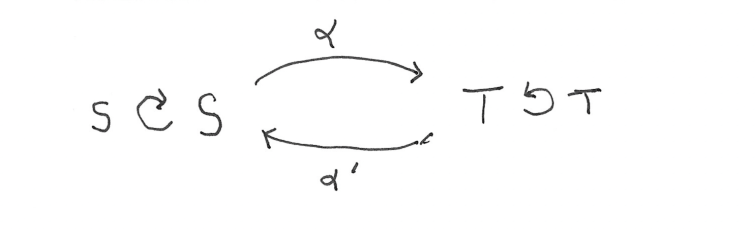
\includegraphics[width=0.6\textwidth]{isomorphism.pdf}
\caption{{\it In a definition adopted from Category Theory, spaces S and T are isomorphic if the diagram commutes, using S and T themselves instead of identity morphisms.}}
\end{figure}

Given a space S, we can identify a number of distinguished classes of morphisms within the semiring of S. 
\begin{itemize}
\item{{\bf Subspaces.} If a morphism $f\in$S happens to also be a space, we say that $f$ is a {\bf subspace} of S.  The name ``subspace'' is justified because every data contained in $f$ is also contained in S, and every morphism $f\cdot$X$\cdot f$ of $f$ is also a morphism of S.  Algebraically, subspaces partially distribute from the left as 
in $f\cdot(g\oplus h)=f\cdot((f\cdot g)\oplus(f\cdot h))$.  In every space, 1, 0 and every constant morphism are subspaces.}
\item {{\bf Neutral Morphisms.} It is easy to see that $0\cdot f=0$ for any $f\in S$.  If $f\cdot 0=0$ also holds, we say that $f$ is a {\it neutral} morphism.  Since 0 and 1 are neutral and since $f\cdot g$ and $f\oplus g$ are neutral if $f$ and $g$ are neutral, neutral morphisms are a sub-semiring of S.} 
\item {{\bf Positive Morphisms.} Morphism $f\in S$ is {\it positive} if ($f$:X)=(0:X) implies (S:X)=(S:).  For example, data D$\in${\bf pass} is positive if D:X=() implies X=().  If $f$ and $g$ are positive, so is $f\cdot g$ and $f\oplus g$, positive morphisms are closed under addition and multiplication. FIX ME}
\item {{\bf Algebraic Morphisms.} The morphisms of an algebraic space are automatically algebraic as well.  In general, if $f,g\in$S and $f$ is algebraic, then $g\cdot f$ is algebraic.  If both 
$f$ and $g$ are algebraic, $f\oplus g$ is algebraic.}
\item{{\bf Homomorphisms.} If a morphism $f$ is distributive, we say that $f$ is a {\bf homomorphism} of S since $f:X\ Y=(f:X)\ (f:Y)$ is a morphism of the main 
structure of S.  Homomorphisms fully distribute from the left as well as the right as in $f\cdot(g\oplus h)=(f\cdot g)\oplus(f\cdot h)$.  Homomorphisms are also closed under 
addition and multiplication, and since 0 and 1 are always homomorphisms, the homomorphisms are a sub-semiring of S.}
\item {{\bf The Group of units}. The collection of morphisms $g\in$S with multiplicative inverses ($g\cdot g'=g'\cdot g=1$) is called {\it the group of units} of the space S.  The group of units may including {\it involutions} where $g\cdot g=1$.  As usual, involutions $g$ and $h$ commute if and only if $g\cdot h$ is also an involution.  Data in S which is invariant under the group of units is 
called {\it central} data.  Morphisms which commute with the group of units are called {\it central} morphisms.}
\end{itemize} 

It is easy to confirm that if spaces S and T are isomorphic as in figure X, it follows a) that $\alpha$ and $\alpha'$ are bijections between the contents of S and the contents of T, b) the semirings of 
S and T are isomorphic as monoids, c) if $\alpha$ and $\alpha'$ are homomorphisms, S and T are also isomorphic as semirings.

\subsection{Subspaces are substructures} 

Suppose space S has subspace $s$ and space T has subspace $t$, and F=$t\cdot X\cdot s$ is a morphism from $s$ to $t$.   Since ($t\cdot X\cdot s$) = ($T\cdot t \cdot X\cdot s\cdot S$), 
F is also a morphism from S to T, with the extra property that F respects the structure of $s$ and $t$ in the sense that $t\cdot F=F\cdot s$.

\begin{figure}[h]
\centering
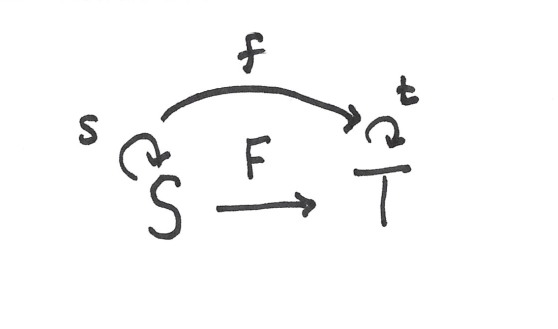
\includegraphics[width=0.3\textwidth]{structure.pdf}
\caption{{\it In a definition adopted from Category Theory, if S with structure $s$ and T with structure $t$ are isomorphic, the top diagram commutes for some morphism $\alpha$ and some morphism $\alpha'$ where S and T function as their own `identity morphisms.' }}
\end{figure}

Since the morphisms of S automatically includes a constant subspace for each data S:X in S, the morphisms of S are strictly richer than the contents of S.  

\subsection{Isomorphisms} 

Spaces S and T are {\bf isomorphic} if the diagram of figure X commutes for some morphisms $\alpha$ and $\alpha'$.  It easily follows that $\alpha$ and $\alpha'$ are bijections between the contents of S and the contents of T and, since $\alpha$ and $\alpha'$ are distributive, S and T are also isomorphic as semirings.



Now we do examples of spaces and their morphisms, growing spaces as organically as possible and aiming for the ``most mathematical'' spaces in the sense of the most algebraic and central.

\section{The Space of pure data} 

     Since idempotents have fixed point images, the only space whose image is all pure data is the identity space {\bf pass}.  Let's examine the structure of {\bf pass} as a space.  From the preorder 
 perspective, {\bf pass}
 \begin{itemize}
 \item{{\bf Subspaces}. Every space S is a subspace {\bf pass}$\cdot$S$\cdot${\bf pass} of {\bf pass}.}
 \item{{\bf Neutral morphisms}. The zero of the semiring of {\bf pass} is, by definition, {\bf pass}$\cdot${\bf null}$\cdot${\bf pass}, which 
 is equal to {\bf null}.  The neutral morphisms of {\bf pass} is the subring of data D satisfying D:X=(). }
 \item{{\bf Positive}. The positive morphisms of {\bf pass} is the subring of data D such that D:X=() implies X=().}
 \item{{\bf Homomorphisms}.  Homomorphisms of {\bf pass} is the subsemiring of distributive data}.
 \item{{\bf Group of units}.  The group of units is the group of sequence permutations such as {\bf swap 1 2} or {\bf rev}.}
 \end{itemize}

The central data are sequences of identical atoms such as (:) (:) (:) or (a a a).  The central morphisms are ap \{a\} etc.  

Isomorphisms with has, has m for any atom m, etc. 

Compare Spaces vs Sets vs Categories 
\begin{itemize}
\item{Unlike sets, spaces cannot be empty.}
\item{Unlike sets, the content of a space does not determine the space.}
\item{Unlike in category theory, every space is a morphism and there are morphisms between any pair of spaces.}  
\item{The set of all sets and the category of all categories is very flaccid.  However the space of all data has lots of structure which is deeply shared.}
\end{itemize}


\begin{figure}[h]
\centering
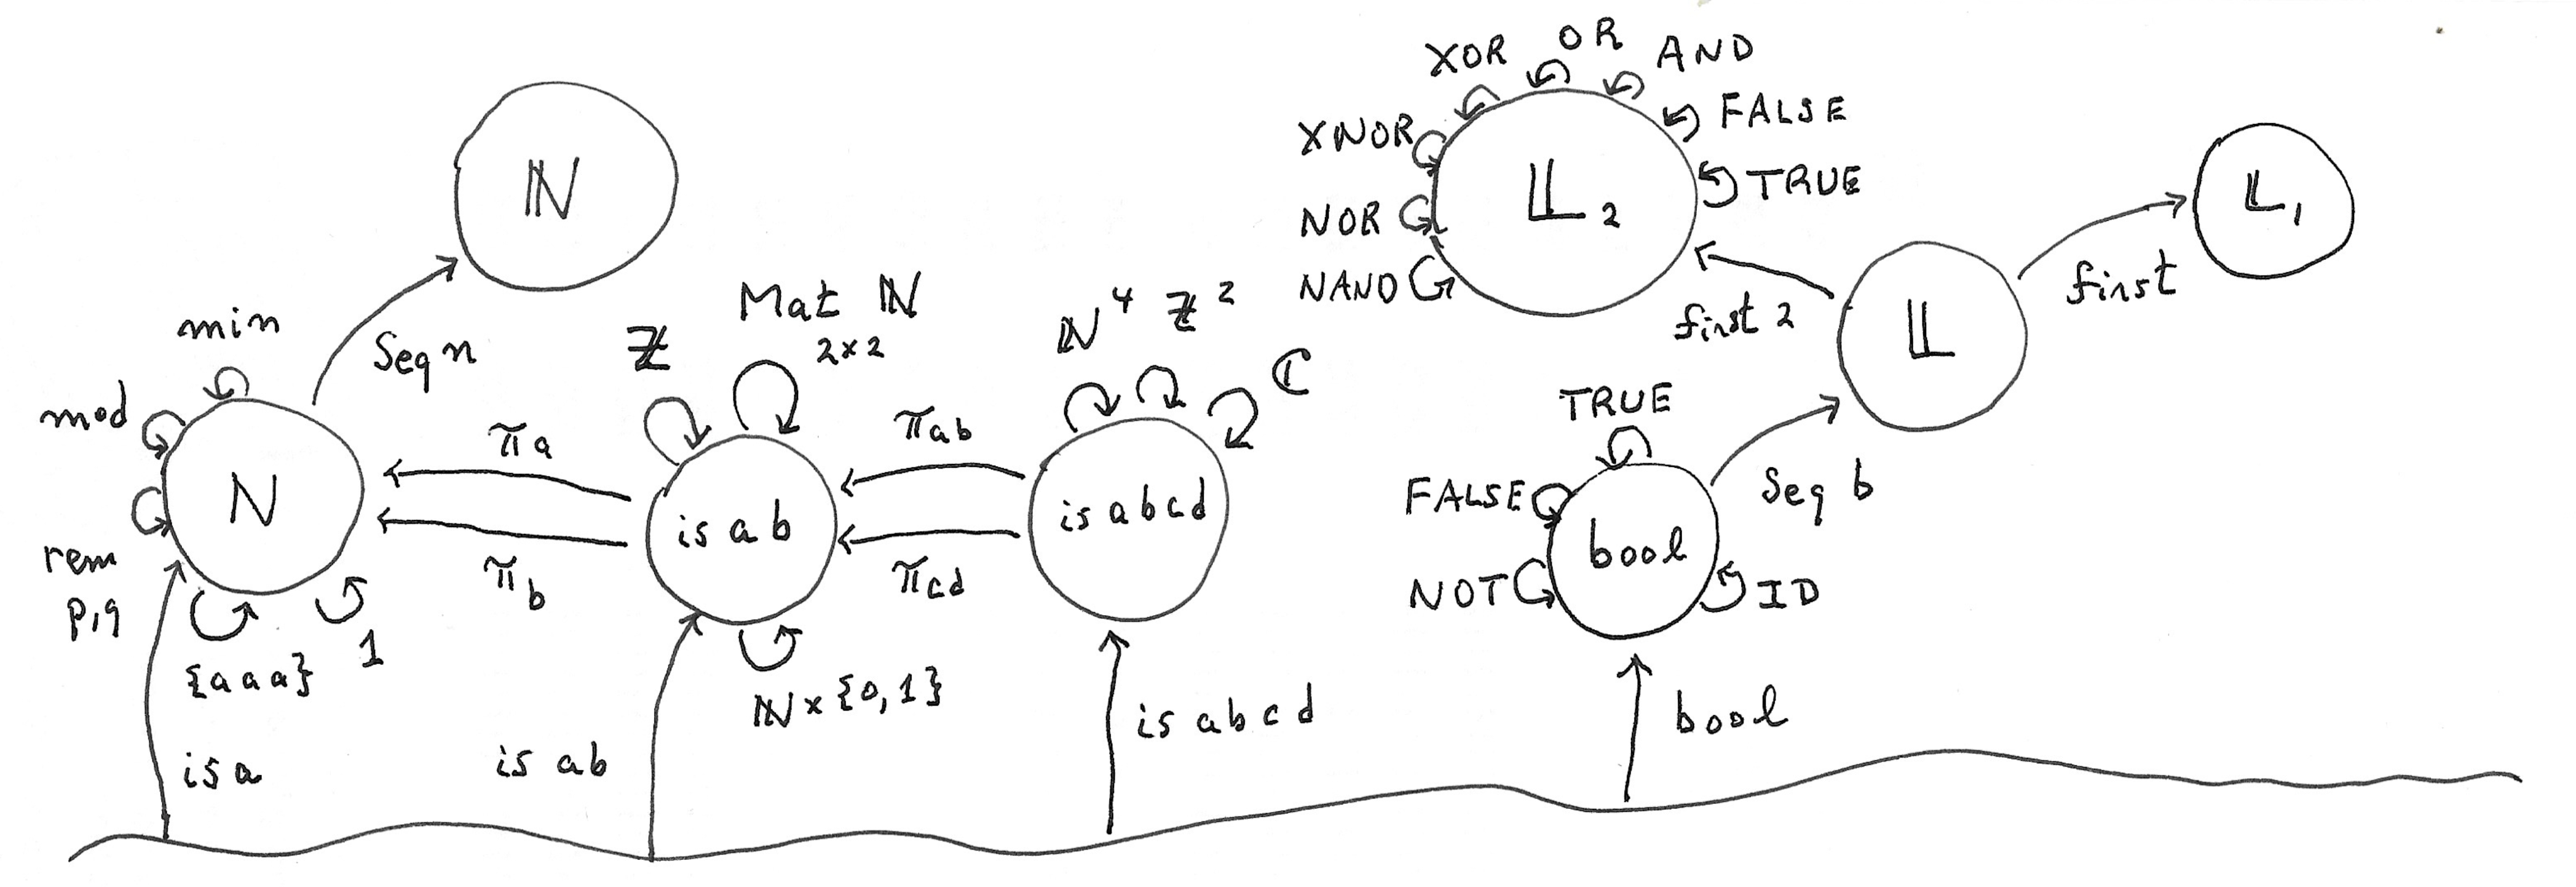
\includegraphics[width=0.7\textwidth]{garden.png}
\caption{{\it Growing spaces ``organically'' from pure data.}}
\end{figure}

\section{Organic Numbers}

      The natural numbers occur most organically simply as sequences of identical atoms, so we might think of (:) (:) (:) or (a a a) as ``3'', depending on a conventional choice of atom.  
Thus, to study natural numbers, we want to find a space N where the data of the space contains all of the natural number lengthed sequences of some chosen atom.  There are many 
spaces which do this, for example,  
\begin{itemize}
\item [1)] The space {\bf atoms} contains all sequences of (:) atoms, (), (:), (:) (:),$\dots$. 
\item [2)] The space {\bf ap const a} contains \{(), a, a a, a a a,$\dots$\}. 
\item [3)] The space {\bf is a}, also containing \{(), a, a a, a a a,$\dots$\}.
\end{itemize}
These are three different spaces.  Choices 1) and 2) are compatible in the preorder sense, however 3) is not compatible with the others and, for instance, has a different kernel.  The main point, however, is that 1) 2) and 3) are isomorphic and they therefore have the same semiring structure.  To be definite, let N be the space ({\bf is a}).  
      
     The first thing to notice about N is that it's main structure is natural number addition, since (N:X Y) is the natural number sum of (N:X) and (N:Y).  Since homomorphisms are distributive, a homomorphism $f$ of N is defined by $f:a$, and thus, $f$ is multiplication by some natural number, for instance, {\bf ap const a a a} is multiplication by 3.  Since these are distributive morphisms, multiplication distributes over addition in N.  Since the group of units is just the identity 1, all of the homomorphisms are central.  
     
    Subspaces of N are indicated by subspace morphisms.  As always, subspace 1 is the whole of N and the subspace 0 consists of just the neutral data of N, which, since in is distributive is the empty sequence.
Besides 0 and 1, it is easy to find two classes of subspaces.  
\begin{itemize} 
\item {\bf Saturation subspaces} An morphism which computes, for example, min($n$,2) such as ({\bf min a a}), is a subspace containing the three data \{(), a, a a\}. 
\item {\bf Modular arithmetic subspaces} An morphism which removes three (a) atoms while possible, such as ({\bf while rem a a a}) is a subspace which computes the sum of it's inputs modulo 3.  Note 
that {\bf while rem a a a} contains the same data as {\bf min a a}, but are not at all the same space. 
\end{itemize}
These two cases can be generalized as follows.  For $p,q\ge 1$, let rem($p$,$q$) be the morphism defined by 
\begin{equation}
{\rm while}\ n\ge p,q: {\rm remove\ p\ from\ n}
\end{equation}
All of these are also subspaces and this generalizes the modular sum and saturation cases since rem($p$,$p$) is $n\mapsto n$ mod $p$ and rem($1$,$q$) is $n\mapsto$ min($n$,$q-1$).   General arguments $p,q\ge 1$.  The rem subspaces are closed under composition via 
\begin{equation}
{\rm rem}(p,q)\cdot {\rm rem}(p',q') = {\rm rem}({\rm lcm}(p,p'),{\rm max}(q,q'))
\end{equation}
so that the rem subspaces are a semilattice.  This completes the subspace analysis of N since every subspace of N is either the whole of N, a constant, or is rem(p,q) for some $p,q\ge1$. 

\begin{proof}
Let $f:{\mathbf N}\rightarrow{\mathbf N}$ where $f(x+y)=f(f(x)+y)=f(x+f(y))$ for all $x,y\in\mathbf N$...
\end{proof}

The most organic generalization of ({\bf is a}) is ({\bf is a b}), which we refer to as N$_2$.  As above, let's consider subspaces.  

\begin{itemize}
\item{The subspaces 1 and 0 give the whole of N$_2$ and just the empty sequence as subspaces, respectively.  
Projections N$_2$$\cdot$({\bf is a})$\cdot$N$_2$ and N$_2$$\cdot$({\bf is b})$\cdot$N$_2$ produce two N-isomorphic subspaces.}
\item{Lexical sorting of N$_2$ sequences is a non-distributive subspace of N$_2$.  Call this endomorphism N.lex, the data of N.lex 
can be written $a^m b^n$ for $m,n\ge 0$.  As in the previous case, a homomorphism M of N.lex is defined by  
\begin{itemize}
\item [] $M: a\mapsto a^{m_{11}} b^{m_{21}}$, and 
\item [] $M: b\mapsto a^{m_{12}} b^{m_{22}}$ 
\end{itemize}
for some choice of 
$
\left (
\begin{array}{cc} 
m_{11} & m_{21} \\ m_{12} & m_{22}  
\end{array}
\right ) 
{\rm in}\ {\rm Mat}_{2\times2}(\mathbf N)
$
where the action of M is exactly matrix multiplication.  Thus, the data of N.lex are pairs of natural numbers the 
homomorphisms are ${\rm Mat}_{2\times2}(\mathbf N)$.  The automorphisms of N.lex are 
$
\left (
\begin{array}{cc} 
1 & 0 \\ 0 & 1 
\end{array}
\right ) 
$
and 
$
\left (
\begin{array}{cc} 
0 & 1 \\ 1 & 0 
\end{array}
\right ) 
$
and the central products are the matrices 
$
\left (
\begin{array}{cc} 
m & n \\ n & m 
\end{array}
\right ) 
$
for $m,n\in\mathbf N$.


}
\item{Reducing data in N$_2$ by removing (a b) and (b a) subsequences defines another subspace (N$_2$.reduce) consisting of 
sequences containing only a's or only b's but not both.  It is easy to see that data in N$_2$.reduce can be identified with the 
integers.  The action of the subspace itself does integer addition.  
The two automorphisms of N$_2$.reduce are the identity and the endomorphism which 
swaps $a\leftrightarrow b$.  A homomorphism $f$ is determined by $f:a$, since $f:b$ is determined by commuting with swap. 
Thus, the central homomorphisms of N$_2$.reduce are exactly integer multiplication, distributing over addition since homomorphisms are 
distributive.  

} 
\end{itemize}

Exploring further in this vein is certainly possible.  It's worth keeping in mind that if spaces commute, their commutator is a new space.  
For instance in {\bf is a b c d}, one can reduce to a subspace by (a b)=(b a)=(c d)=(d c)=1, this reduction commutes with a lexical sort 
and so the two can be composed to create $\mathbf Z\times\mathbf Z$ with homomorphisms ${\rm Mat}_{2\times2}(\mathbf N)$.  
More generally, any confluent convergent rewrite system on some chosen alphabet is automatically a space and could be subject to similar analysis. 

\begin{proof}
....
\end{proof}

\subsection{Number Sequences}

      Given the space N from the previous section, let {$\mathbb N$} be 
\begin{equation}
{{\bf ap}\ ({\bf put\ n})\cdot N \cdot ({\bf get\ n})}
\end{equation}
where {\bf n} is some chosen atom.  Since $({\bf put\ n})\cdot N \cdot ({\bf get\ n})$ is idempotent, ${\mathbb N}$ is a distributive space containing 
sequences of n-atoms containing N-data, such as 
\begin{itemize}
\item[] T = (n:a a a) (n:) (n:a a) (n:a) (n:)
\end{itemize} 

Unlike the case of N, the action of ${\mathbb N}$ is merely to concatenate sequences.  It's easy, however, to identify 
natural number sum again as one of several subspaces 
\begin{itemize}
\item sum:T = (n:a a a a a a)
\item sort:T = (n:) (n:) (n:a) (n:a a) (n:a a a)
\item min:T = (n:)
\item max:T = (n:a a a)
\item first:T = (n:a a a)
\end{itemize} 
All but the last are algebraic subspaces are therefore ``more mathematical.''   Consider a morphism from 

Some of the morphisms of ${\mathbb N}$ are ``inherited'' from $f\in$N.  Define {\bf inner}:F to be 
\begin{equation}
{\mathbb N}\cdot({\rm put\ n})\cdot F\cdot({\rm get\ n})\cdot{\mathbb N}
\end{equation}
so that ({\bf inner}:F):X means letting F act on the concatenated N-contents of X, returning the result in a single n-atom.  The sum morphism 
above, for instance, is equal to inner:N.  The construction (5) and (6) works for any space, not just for S and so if we define a ``functor'' {\bf Seq} 
to be 
\begin{equation}
({\rm put}\ {\rm A})\cdot {\rm B} \cdot ({\rm get}\ {\rm A})
\end{equation}
Then {$\mathbb N$} is equal to (Seq n:N) and given any atom s and any space S, (Seq s:S) is the space of S-values stored in s-atoms.  
Similarly, if we define {\bf inner} to be  
\begin{equation}
{\mathbb N}\cdot\{({\rm put\ n})\cdot{\rm B}\cdot({\rm get\ n})\}\cdot{\mathbb N}
\end{equation}
then inner:F is the inner version of F$\in$S.  Other general constructions of this type are possible.  For example, let {\bf series} be 
\begin{equation}
{\mathbb N}\cdot\{{\rm B\ (A:B)}\}\cdot{\mathbb N} 
\end{equation}
and, thus (series:F) applies F to data appending the result.  For example, the morphism {\bf series}$\cdot$({\bf inner}:{\bf back a a}) 
generates the Fibbonacci sequence (n:a) (n:a) (n:a a) (n:a a a)$\dots$.

Summarize...

\section{Boolean} 

      The space {\bf bool} is algebraic and positive, but not distributive.  Since {\bf bool} contains two data:  () for {\it true} and (:) for {\it false},   
 there are only four morphisms:  ID={\bf bool},  the constants TRUE=\{\} and FALSE=\{(:)\}, and one involution 
 NOT={\bf bool}$\cdot${\bf not}$\cdot$.  The morphism semiring is explicit in Table X, where it's useful to note that $\oplus$ is commutative since {\bf bool} is 
 algebraic, and $f\oplus f=f$ for $f\in${\bf bool}.  

The subspaces of {\bf bool} are ID, TRUE and FALSE, so {\bf bool} has only trivial subspaces.  The morphisms ID and TRUE are neutral, ID is the only positive 
morphism and all morphisms are algebraic since {\bf bool} itself is algebraic.  The group of units is ID and NOT and ID is the only central morphism. 

\begin{table}
\begin{tabular}{| l | l | l | l | l |  }
$f\cdot g$ & ID & TRUE & FALSE & NOT  \\
\hline
ID &  ID & TRUE & FALSE &  NOT \\
TRUE & TRUE & TRUE  & TRUE & TRUE \\
FALSE & FALSE  & FALSE & FALSE & FALSE   \\
NOT & NOT & FALSE & TRUE & ID \\
\hline
\end{tabular}
\begin{tabular}{| l | l | l | l | l |  }
$f\oplus g$ & ID & TRUE & FALSE & NOT  \\
\hline
ID &  ID & ID & FALSE & FALSE \\
TRUE & - & TRUE  & FALSE & NOT \\
FALSE & -  & - & FALSE & FALSE   \\
NOT & - & - & - & NOT \\
\hline
\end{tabular}
\caption{{\it Product and sum of the four morphisms ID, TRUE, FALSE, NOT of the space {\bf bool}}.  Note that ID is the unit of multiplication and TRUE is the 
unit of addition, and we have $f\oplus g=g\oplus f$, since {\bf bool} is algebraic, and $f\oplus f=f$.}
\end{table}

\subsection{Boolean Sequences}

As in the case of N, we can let $\mathbb L$=(Seq b:bool), be the distributive space of bool-valued data stored in b-atoms, so a typical data in $\mathbb L$ is 
\begin{equation}
{\rm (b:)\ (b:)\ (b:(:))\ (b:)\ (b:(:))\ (b:(:))}
\end{equation}
Let's agree to write such sequences replacing (b:) with T, (b:(:)) with F and the empty sequence with 0, so that the above is written TTFTFF.   
Let's also consider the shortest subspaces of $\mathbb L$ first.  The space morphism {\bf first}$\in\mathbb L$ are the sequences of length at most 1.  
Let's call this space ${\mathbb L}_1$ and, similarly, let ${\mathbb L}_2$ be (first 2)$\in\mathbb L$.  Thus, ${\mathbb L}_1$ contains data \{0,T,F\} and ${\mathbb L}_2$ contains data \{0,T,F,TT,TF,FT,FF\}. 
Since ${\mathbb L}_1$ has 27 morphisms and ${\mathbb L}_2$ already has $7^7=823,543$ morphisms, ${\mathbb L}_1$ is the last chance to be complete and explicit.  
For ${\mathbb L}_1$, we can specify a morphism $f\in {\mathbb L}_1$ by listing the values of $f$ on 0,T,F in standard order, so 0TF is the identity morphism, etc.  
Figure X shows the 27 morphisms showing that even in a small space like ${\mathbb L}_1$, all the categories of morphisms appear in a nontrivial way.  

    Consider, at least, the inner morphisms of ${\mathbb L}_2$.  These are the morphisms of the form
 \begin{equation}
 {\mathbb L}_2\cdot ({\bf put}\ b)\cdot F \cdot ({\bf get}\ b) \cdot {\mathbb L}_2 
 \end{equation}
 where $F$ can be any data.  Since ({\bf get}\ b):X only depends on the number of (:) values in the b-atoms of X and since the morphism always produces exactly one b-atom, 
 there are eight inner morphismsas shown in \cite{L2}.

\begin{figure}[h]
\centering
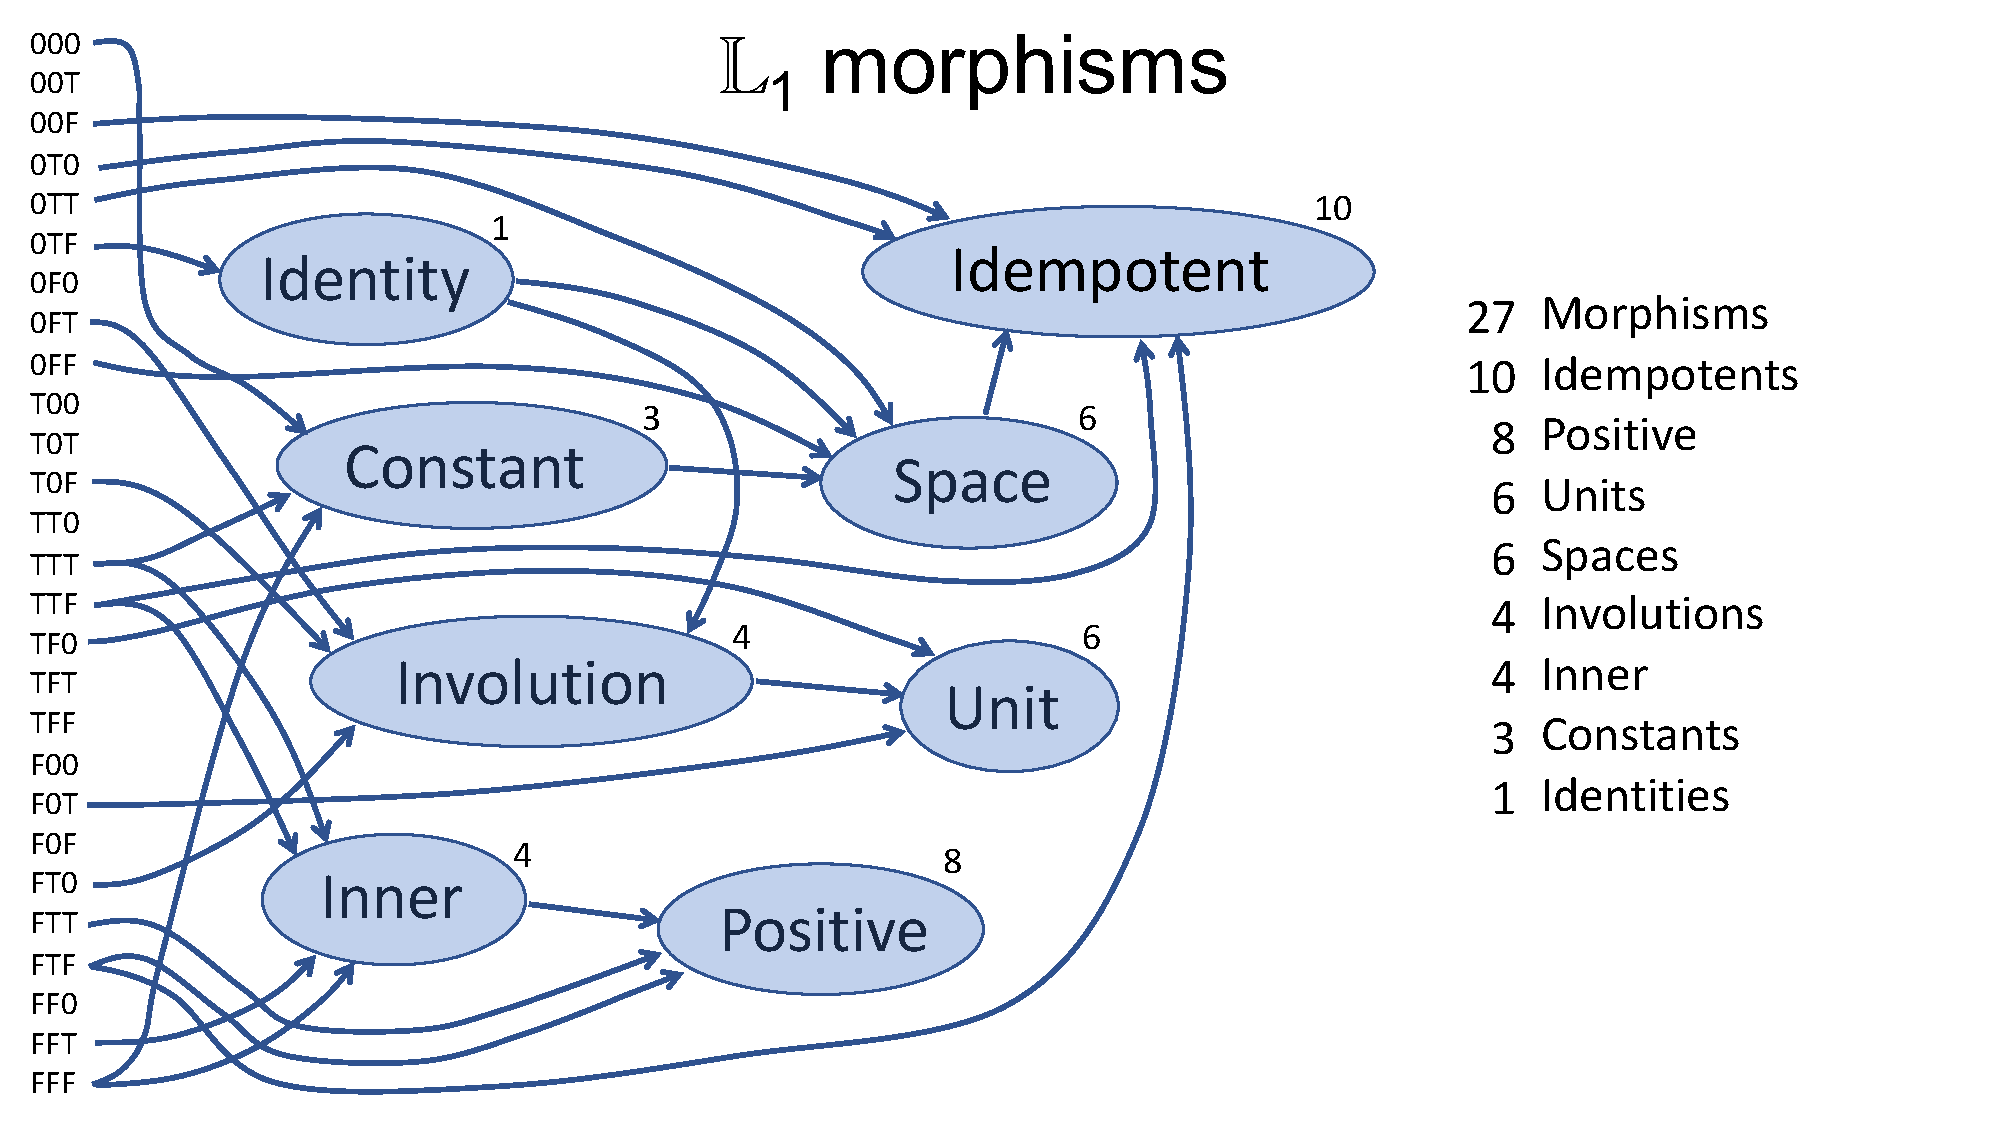
\includegraphics[width=0.8\textwidth]{L1.pdf}
\caption{{\it Morphisms of ${\mathbb L}_1$.}}
\end{figure}

\begin{table}
\caption{The eight inner morphisms of ${\mathbb L}_2$ slightly generalize the eight standard symmetric binary boolean operators.}
\centering 
\begin{tabular}{r c c c c c c c r r l}
\hline\hline
$e_i \in {\mathbb L}_2$ & 0 & T & F & TT & TF & FT & FF & standard & generalized & description \\ [0.5ex] 
\hline
$e_1$  & T & T & T & T & T & T & T & TRUE & {\bf always} & always true \\
$e_2$  & T & T & T & T & T & T & F & OR & {\bf any} & any are true \\
$e_3$  & T & T & F & T & F & F & T & XNOR & {\bf even} & even (:)s \\
$e_4$ & T & T & F & T & F & F & F & AND & {\bf all} & all are true \\
$e_5$ & F & F & T & F & T & T & T & NAND & {\bf notall} & not all are true \\
$e_6$ & F & F & T & F & T & T & F & XOR & {\bf odd} & odd (:)s \\
$e_7$ & F & F & F & F & F & F & T & NOR & {\bf none} & none are true  \\
$e_8$ & F & F & F & F & F & F & F & FALSE & {\bf never} & never true \\
\hline
Number of (:)   & 0 & 0 & 1 & 0 & 1 & 1 & 2 &  \\ 
\hline
\end{tabular}
\label{table:L2}
\end{table} 

\begin{figure}[h]
\centering
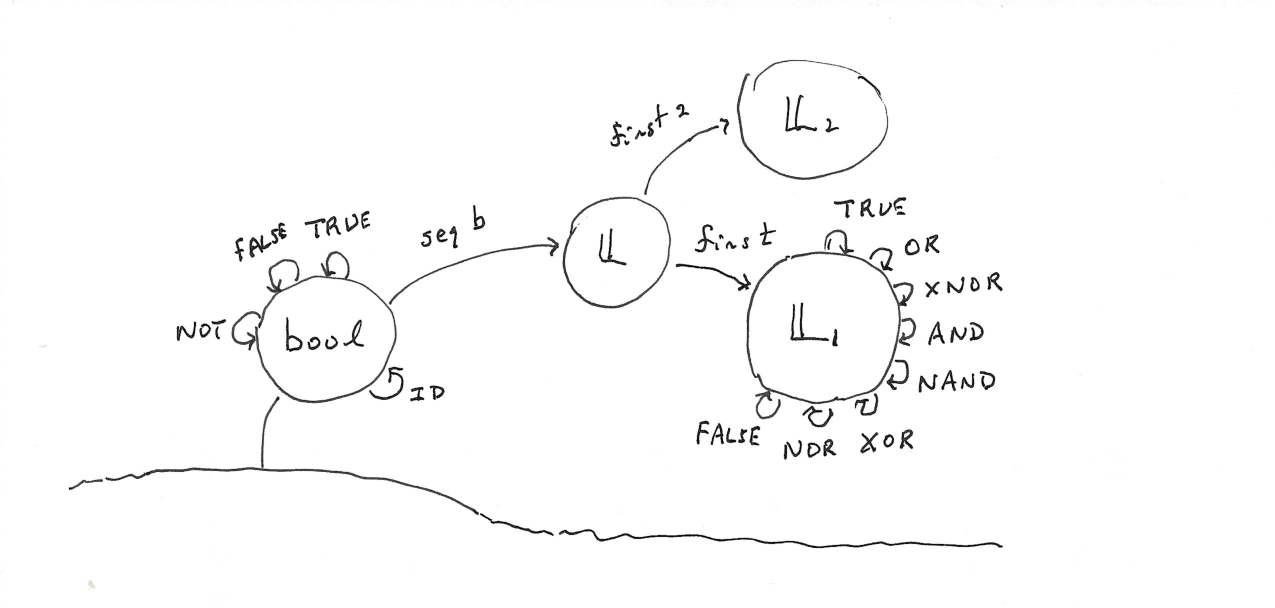
\includegraphics[width=0.8\textwidth]{bool.pdf}
\caption{{\it In a definition adopted from Category Theory, if S with structure $s$ and T with structure $t$ are isomorphic, the top diagram commutes for some morphism $\alpha$ and some morphism $\alpha'$ where S and T function as their own `identity morphisms.' }}
\end{figure}

\begin{figure}[h]
\centering
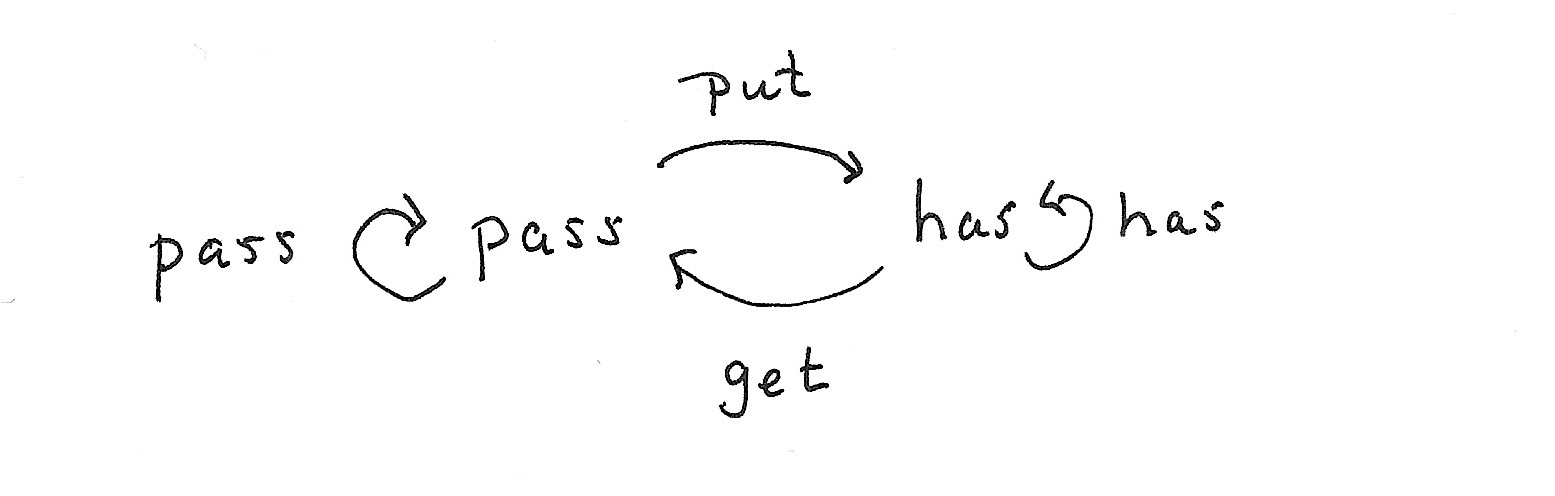
\includegraphics[width=0.6\textwidth]{Pass-has.png}
\caption{{\it In a definition adopted from Category Theory, if S with structure $s$ and T with structure $t$ are isomorphic, the top diagram commutes for some morphism $\alpha$ and some morphism $\alpha'$ where S and T function as their own `identity morphisms.' }}
\end{figure}

\begin{figure}[h]
\centering
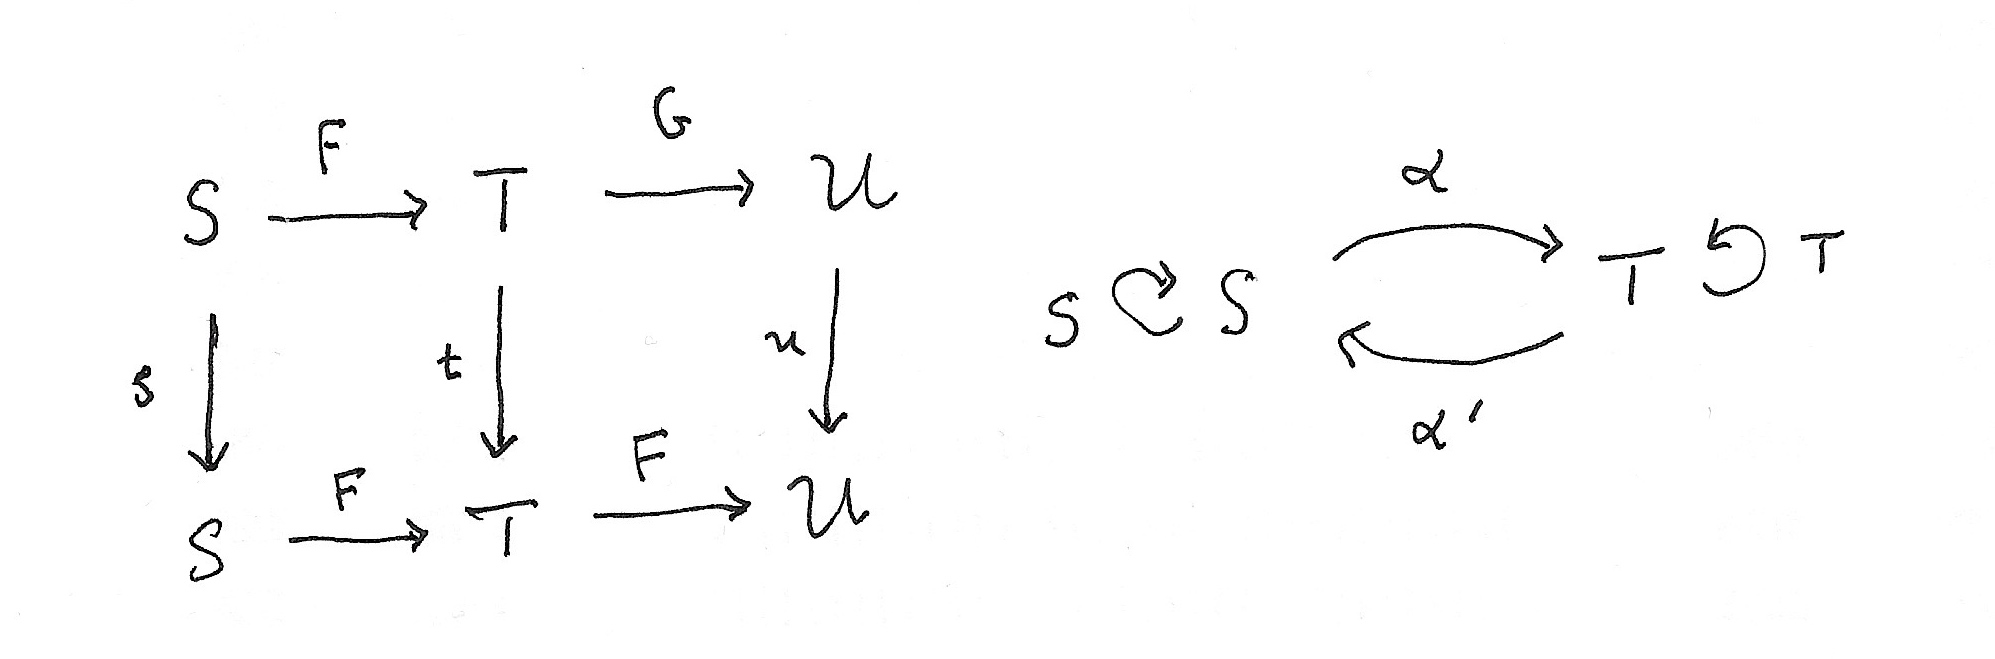
\includegraphics[width=0.7\textwidth]{Morphisms.png}
\caption{{\it The diagram on the left demonstrates that S${\overset F\longrightarrow}$T and T${\overset G\longrightarrow}$U implies $S{\overset {G\cdot F} \longrightarrow}$U, where space S has structure $s$, space T has structure $t$, and space U has structure $u$.  Spaces S and T are said to be isomorphic, if the diagram on the right commutes for some morphisms $\alpha$ and $\alpha'$.}}
\end{figure}

Figure 2 illustrates these definitions and demonstrates that composition of morphisms is associative.  If S${\overset F\longrightarrow}$T and T${\overset G\longrightarrow}$U, then S${\overset {G\cdot F} \longrightarrow}$U, where S, T and U are spaces (with structure).  Figure 2 also illustrates how 
definitions can be adopted from Category Theory.  For example, we say that spaces S and T are {\bf isomorphic} if the diagram of Figure 2(c) commutes for some morphisms $\alpha$ and $\alpha'$, denoted by S${\overset \alpha \cong}$T.  

\section{Glossary}

For example, starting with context $\delta$, we can add more atoms of the form $\delta_a:c\mapsto c$:
\begin{enumerate}
\item[-]{$\delta_{(:)}$ : ((:) A : B) $\mapsto$ ((:) A : B), {\it single bit atoms where ((:):), ((:):(:)) are zero,one respectively.}}
\item[-]{$\delta_{((:):)}$ : (((:):) A : B) $\mapsto$ (((:):) A : B), {\it eight bit bytes.}}
\item[-]{$\delta_{((:):(:))}$ : (((:):(:)) A : B) $\mapsto$ (((:):(:)) A : B), {\it byte sequences}.}
\end{enumerate}
so that text strings or other data are atomic data within $\delta\cup\delta_{(:)}\cup\delta_{((:):)}\cup\delta_{((:):(:))}$.  We can then proceed to add named 
definitions that `get coda components':
\begin{enumerate}
\item[-]{$\delta_{\bf pass}$ : ({\bf pass} A:B) $\mapsto$ B}
\item[-]{$\delta_{\bf null}$ : ({\bf null} A:B) $\mapsto$ ()}
\item[-]{$\delta_{\bf right}$ : ({\bf right} A:B) $\mapsto$ B} 
\item[-]{$\delta_{\bf arg}$ : ({\bf arg} A:B) $\mapsto$ A} 
\end{enumerate}
and can add definitions for simple combinatorics 
\begin{enumerate}
\item[-]{$\delta_{\bf ap}$ : ({\bf ap} A : b B) $\mapsto$ (A:b) (ap A:B), {\it apply A to each atom in B.}}
\item[-]{$\delta_{\bf rev}$ : ({\bf rev} A : B b) $\mapsto$ b (rev : B), {\it reverse the order of atoms in B.}}
\end{enumerate}

definitions computing the boolean value of data 
\begin{enumerate}
\item[-]{$\delta_{\bf bool}$ : ({\bf bool} A : B b) $\mapsto$ () if B is empty, (:) if B is atomic, {\it logical value of B.}}
\end{enumerate}
definitions making new definitions  
\begin{enumerate}
\item[-]{$\delta_{\bf def}$ : ({\bf def} a : B) $\mapsto$ Add $\delta_a$ to context if $a$ is an unused invariant atom.} 
\end{enumerate}
As explained in reference \cite{PDF}, a language is introduced merely as one more definition where the domain of the language context $\delta_{\{\}}$ is 
codas starting with a curly brace as in (\{{\it language expression}\} A : B).  
\begin{enumerate}
\item[-]{$\delta_{\bf bool}$ : ({\bf bool} A : B b) $\mapsto$ () if B is empty, (:) if B is atomic, {\it logical value of B.}}
\end{enumerate}
definitions making new definitions  
\begin{enumerate}
\item[-]{$\delta_{\bf def}$ : ({\bf def} a : B) $\mapsto$ Add $\delta_a$ to context if $a$ is an unused invariant atom.} 
\end{enumerate}
As explained in reference \cite{PDF}, a language is introduced merely as one more definition where the domain of the language context $\delta_{\{\}}$ is 
codas starting with a curly brace as in (\{{\it language expression}\} A : B).  

%%%%%%%%%%%%%%%%%%%%%%%%%%%%%%%%%%%%%%%%%%%%%%%%%%%%%%%%%%%%%%%%%%%%%%%%
%%% \bibliography{jpsi}
\begin{thebibliography}{10}
\bibitem{PDF} {\it Pure Data Foundation of Mathematics and Computing}, Saul Youssef, 2023.
\bibitem{Berry} Nicholas Griffin (2003-06-23). {\it The Cambridge Companion to Bertrand Russell}. Cambridge University Press. p. 63. ISBN 978-0-521-63634-6.
\bibitem{Mazur} Barry Mazur, {\it When is one thing equal to some other thing?}, Harvard University, 2007,  {\rm https://people.math.harvard.edu/}$\sim${\rm mazur/preprints/when\_is\_one.pdf}. 
\end{thebibliography}
%%%%%%%%%%%%%%%%%%%%%%%%%%%%%%%%%%%%%%%%%%%%%%%%%%%%%%%%%%%%%%%%%%%%%%%%
\end{document}
